\section{一维传播公式}
\label{sec:wave-dalembert}

无界的弦上没有端点干扰，一维波动问题可以完全解出来。解的公式会回答两个问题：初始位移和初始速度各起什么作用，某一时空点的值究竟取决于哪段初值。

\paragraph{换坐标：沿两族直线看}
第~\ref{chap:pde-problems}章指出，一维波动方程的特征线是两族直线$x\pm ct=$常数。沿这两族直线取坐标，方程会变得非常简单。令
\[
 \xi=x-ct,\qquad \eta=x+ct,
\]
并把$u$写成$(\xi,\eta)$的函数。由链式法则，
\[
 \partial_x=\partial_\xi+\partial_\eta,\qquad \partial_t=c(\partial_\eta-\partial_\xi).
\]

把这两个算子分别平方再作差，混合项是唯一留下的部分：
\[
 \partial_t^{2}-c^{2}\partial_x^{2}=c^{2}(\partial_\eta-\partial_\xi)^{2}-c^{2}(\partial_\xi+\partial_\eta)^{2}=-4c^{2}\partial_\xi\partial_\eta .
\]
于是无源的波动方程等价于
\begin{equation}
 \partial_\xi\partial_\eta u=0.
 \label{eq:wave-characteristic-form}
\end{equation}

式~\eqref{eq:wave-characteristic-form}说$\partial_\eta u$不随$\xi$变化，只是$\eta$的函数。对$\eta$积分，积分“常数”是$\xi$的函数。所以$C^{2}$解都可以写成两个一元函数之和：
\begin{equation}
 u(x,t)=F(x-ct)+G(x+ct).
 \label{eq:wave-general-solution}
\end{equation}

$F(x-ct)$是形状$F$以速度$c$向右平移，$G(x+ct)$是形状$G$以速度$c$向左平移。这两项称为\term{行波}（travelling wave）。方程$\partial_t^{2}u=c^{2}\partial_x^{2}u$的全部解都由一列右行波和一列左行波叠加而成，两列波互相穿过，彼此不改变形状。

\paragraph{由初值确定两列波}
把式~\eqref{eq:wave-general-solution}代入两个初始条件，得到
\[
 F(x)+G(x)=u_0(x),\qquad -cF'(x)+cG'(x)=u_1(x).
\]
对第二式从$0$到$x$积分，再除以$c$，其中$K=G(0)-F(0)$是常数：
\[
 G(x)-F(x)=\frac1c\int_0^{x}u_1(s)\,\mathrm{d}s+K .
\]

把它与第一式相加减，就解出了两个函数：
\[
 \begin{aligned}
  F(x)&=\frac12u_0(x)-\frac1{2c}\int_0^{x}u_1(s)\,\mathrm{d}s-\frac K2,\\
  G(x)&=\frac12u_0(x)+\frac1{2c}\int_0^{x}u_1(s)\,\mathrm{d}s+\frac K2 .
 \end{aligned}
\]
代回式~\eqref{eq:wave-general-solution}，常数$K$相消，两个积分合并成从$x-ct$到$x+ct$的积分。这样就得到了下面的公式。

\begin{theorem}[\term{d'Alembert公式}（d'Alembert formula）]
\label{thm:wave-dalembert}
设$u_0\in C^{2}(\mathbb{R})$，$u_1\in C^{1}(\mathbb{R})$。一维问题$\partial_t^{2}u=c^{2}\partial_x^{2}u$，$u(\cdot,0)=u_0$，$\partial_tu(\cdot,0)=u_1$在$\mathbb{R}\times[0,\infty)$上有唯一的$C^{2}$解
\begin{equation}
 u(x,t)=\frac12\bigl[u_0(x-ct)+u_0(x+ct)\bigr]+\frac1{2c}\int_{x-ct}^{x+ct}u_1(s)\,\mathrm{d}s .
 \label{eq:wave-dalembert}
\end{equation}
\end{theorem}

\begin{proof}
先证唯一性。设$u$是$C^{2}$解，换到坐标$(\xi,\eta)$后，$t\geq0$对应区域$\eta\geq\xi$。这个区域在两个坐标方向上的截线都是连通的半直线，所以式~\eqref{eq:wave-characteristic-form}可以如上逐次积分，得到式~\eqref{eq:wave-general-solution}。前面的代入过程说明$F,G$由初值确定到相差一个相消的常数，因此$u$必定是式~\eqref{eq:wave-dalembert}。

再证式~\eqref{eq:wave-dalembert}确实是解。记$x_-=x-ct$，$x_+=x+ct$。由链式法则和变上限积分的求导公式，对$x$求两次，得到
\[
 \partial_x^{2}u=\frac12\bigl[u_0''(x_-)+u_0''(x_+)\bigr]+\frac1{2c}\bigl[u_1'(x_+)-u_1'(x_-)\bigr].
\]

对$t$求一次，$x_\pm$对$t$的导数是$\pm c$，于是
\[
 \partial_tu=\frac c2\bigl[-u_0'(x_-)+u_0'(x_+)\bigr]+\frac12\bigl[u_1(x_+)+u_1(x_-)\bigr].
\]

再对$t$求一次，得到
\[
 \partial_t^{2}u=\frac{c^{2}}2\bigl[u_0''(x_-)+u_0''(x_+)\bigr]+\frac c2\bigl[u_1'(x_+)-u_1'(x_-)\bigr].
\]
比较前后两式，$\partial_t^{2}u=c^{2}\partial_x^{2}u$。题设的光滑性保证这些导数都连续。令$t=0$，$x_-=x_+=x$，积分项为零，$u=u_0$；$\partial_tu$的表达式给出$\partial_tu=u_1$。
\end{proof}

用一组光滑的数据验证公式。取$c=2$，$u_0=\sin x$，$u_1=\cos x$。式~\eqref{eq:wave-dalembert}的两项分别是
\[
 \begin{aligned}
  \frac12\bigl[\sin(x-2t)+\sin(x+2t)\bigr]&=\sin x\cos2t,\\
  \frac14\int_{x-2t}^{x+2t}\cos s\,\mathrm{d}s&=\frac12\cos x\sin2t .
 \end{aligned}
\]
两者之和满足$\partial_t^{2}u=-4u=4\partial_x^{2}u$，$t=0$时位移是$\sin x$，速度是$\cos x$。

式~\eqref{eq:wave-dalembert}有两项，分别来自初始位移和初始速度。由线性性，可以把它们分开讨论。

\paragraph{初始位移的贡献}
取$c=1$，初速度为零，初始位移是帐篷形
\[
 u_0(x)=\Lambda(x)=\max\{1-\lvert x\rvert,\,0\}.
\]
式~\eqref{eq:wave-dalembert}只剩第一项，解是
\begin{equation}
 u(x,t)=\frac12\bigl[\Lambda(x-t)+\Lambda(x+t)\bigr].
 \label{eq:wave-tent-solution}
\end{equation}
帐篷在$0,\pm1$处有折角，严格说来不是$C^{2}$函数，式~\eqref{eq:wave-tent-solution}在折角运动的线上没有二阶导数，它是第~\ref{chap:pde-problems}章意义下的弱解，可以看成光滑初值的解的极限。

式~\eqref{eq:wave-tent-solution}说，初始鼓包分成高度减半的两份，一份向右，一份向左。取$t=1/2$，手算几个点的值：
\[
 \begin{aligned}
  u(0,\tfrac12)&=\tfrac12[\Lambda(-\tfrac12)+\Lambda(\tfrac12)]=\tfrac12,\\
  u(\tfrac12,\tfrac12)&=\tfrac12[\Lambda(0)+\Lambda(1)]=\tfrac12,\\
  u(1,\tfrac12)&=\tfrac12[\Lambda(\tfrac12)+\Lambda(\tfrac32)]=\tfrac14 .
 \end{aligned}
\]
此时两份还重叠着，叠加成高度$1/2$的平台。到$t=1$，两份恰好分开；到$t=2$，它们的中心分别在$\pm2$，中间的弦回到零位，如图~\ref{fig:wave-dalembert-displacement}。

\begin{BookInlineFigure}
  \centering
  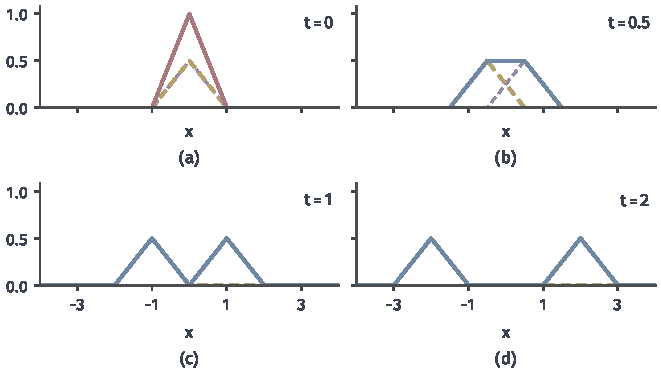
\includegraphics[width=112mm]{figures/06-differential-equations/02-partial-differential-equations/matplotlib/wave-dalembert-displacement/figure.pdf}
  \caption{帐篷形初始位移（$c=1$，初速度为零）在四个时刻的解。黄色虚线是左行波$\frac12\Lambda(x+t)$，紫色虚线是右行波$\frac12\Lambda(x-t)$，实线是两者之和。鼓包分成两半后互不干扰，形状和高度此后不再改变。}
  \label{fig:wave-dalembert-displacement}
\end{BookInlineFigure}

注意帐篷的折角也被带走了。原来的三个折角各分裂成两个，分别沿特征线运动，没有任何一个被磨圆。对比热方程，折角在任意正时刻都消失。波动方程的解在时刻$t$和初值一样光滑，不会更光滑。

\paragraph{初始速度的贡献}
再取初始位移为零，用小锤敲打区间$(-1,1)$，即$c=1$，$u_1=\mathbb{I}\{\lvert x\rvert<1\}$。式~\eqref{eq:wave-dalembert}只剩积分项，被积函数只在$(-1,1)$上不为零，所以
\begin{equation}
 u(x,t)=\frac12\,\bigl\lvert(x-t,\,x+t)\cap(-1,1)\bigr\rvert .
 \label{eq:wave-box-solution}
\end{equation}
竖线表示区间的长度。这个函数连续，但$u_1$的跳跃使它不是$C^{2}$函数，它同样在弱的意义下解方程。

固定一个位置观察。在$x=0$处，式~\eqref{eq:wave-box-solution}的交集在$t\leq1$时是$(-t,t)$，在$t\geq1$时是$(-1,1)$，于是
\[
 u(0,t)=\min\{t,\,1\}.
\]
位移先线性上升，到$t=1$后停在$1$，再也不回来。

固定一个时刻观察。取$t=3$，在几个点上读出交集的长度：
\[
 u(0,3)=\tfrac12\cdot2=1,\qquad u(3,3)=\tfrac12\cdot1=\tfrac12,\qquad u(4,3)=0.
\]
解是一个梯形：在$\lvert x\rvert\leq t-1$上高度为$1$，在$\lvert x\rvert=t+1$处降到零。图~\ref{fig:wave-dalembert-velocity}显示这个梯形不断变宽，高度不变。

\begin{BookInlineFigure}
  \centering
  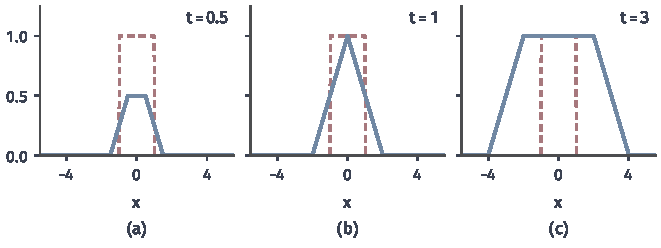
\includegraphics[width=112mm]{figures/06-differential-equations/02-partial-differential-equations/matplotlib/wave-dalembert-velocity/figure.pdf}
  \caption{初始速度为$(-1,1)$的指示函数（红色虚线）时三个时刻的解（蓝），$c=1$，初始位移为零。解是逐渐变宽的梯形，中间的平台高度为$1$，$t>1$后不再升高。}
  \label{fig:wave-dalembert-velocity}
\end{BookInlineFigure}

为什么速度的贡献是积分？设想只在一点$y$附近的小区间$\mathrm{d}y$上有初速度。式~\eqref{eq:wave-dalembert}的积分说，$\lvert x-y\rvert<ct$的点得到位移$u_1(y)\,\mathrm{d}y/(2c)$，更远的点还没有收到信号。一次局部的推动在波前走过的范围内留下固定的抬高，所有$y$的贡献加起来就是积分。

这和初始位移的情形不同。位移的两半走开后，中间恢复零位；速度的作用却留下永久的位移，因为被敲过的弦有净动量。对空间积分可以把这件事算清楚。由式~\eqref{eq:wave-box-solution}，$\int_{\mathbb{R}}\partial_tu\,\mathrm{d}x$保持为初值的积分$2$，所以
\[
 \int_{\mathbb{R}}u(x,t)\,\mathrm{d}x=2t.
\]
梯形的面积正是这样增长的：宽度每单位时间增加$2$，高度为$1$。

\paragraph{一个时空点依赖哪段初值}
式~\eqref{eq:wave-dalembert}直接告诉我们计算$u(x_0,t_0)$要用到什么：$u_0$只用到两个端点$x_0\pm ct_0$，$u_1$用到整个区间$[x_0-ct_0,x_0+ct_0]$。从点$(x_0,t_0)$沿两条特征线回溯到$t=0$，就截出这个区间，如图~\ref{fig:wave-dependence}(a)。

反过来，初值在区间$[a,b]$上的变化只能影响图~\ref{fig:wave-dependence}(b)的阴影区域，$a-ct\leq x\leq b+ct$，以外的点完全不受影响。扰动以速度$c$向两侧扩展。

\begin{BookInlineFigure}
  \centering
  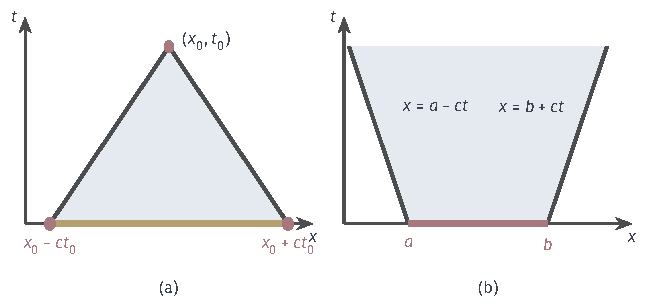
\includegraphics[width=109.647mm]{figures/06-differential-equations/02-partial-differential-equations/tikz/wave-dependence/figure.pdf}
  \caption{一维波动方程的依赖关系。(a)点$(x_0,t_0)$的值由两条特征线（深灰）截出的区间决定：两个红点是所用的位移，黄色线段是所用的速度。(b)初始数据$[a,b]$（红色线段）的变化只能影响阴影区域。}
  \label{fig:wave-dependence}
\end{BookInlineFigure}

用前面的两个例子走一遍。取$c=1$，$(x_0,t_0)=(1/2,2)$，依赖区间是$[-3/2,5/2]$。帐篷初始位移只用到$u_0(-3/2)$和$u_0(5/2)$，两者都为零，于是
\[
 u(\tfrac12,2)=0.
\]
帐篷的两半都已经从这里经过。小锤初始速度要用整个依赖区间，其中包含$(-1,1)$，于是
\[
 u(\tfrac12,2)=\tfrac12\cdot2=1.
\]
如果把初值在$x=3$附近改掉，这两个数都不变，因为$3$不在依赖区间内。

图~\ref{fig:wave-spacetime}把两个例子画在时空平面上。(a)中的折角沿特征线运动，帐篷走后留下空白；(b)中两列波前沿之间的弦保持抬高。

\begin{BookInlineFigure}
  \centering
  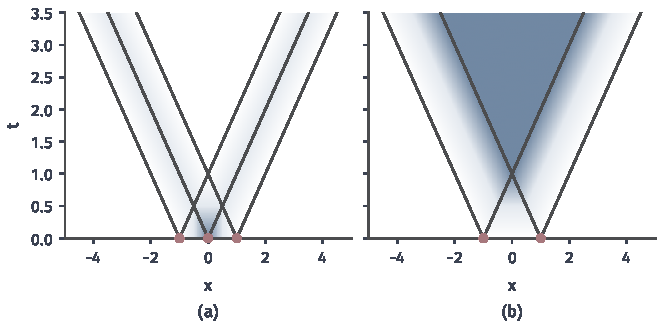
\includegraphics[width=112mm]{figures/06-differential-equations/02-partial-differential-equations/matplotlib/wave-spacetime/figure.pdf}
  \caption{时空平面上的解，$c=1$，颜色越深$u$越大。(a)帐篷形初始位移。(b)$(-1,1)$上的初始速度。深灰直线是从初始数据的折点（红点）出发的特征线，解的不光滑处全部落在这些线上。}
  \label{fig:wave-spacetime}
\end{BookInlineFigure}

\paragraph{解对初值的连续依赖}
由式~\eqref{eq:wave-dalembert}，把两项分别放大，得到点态估计
\begin{equation}
 \sup_{x}\lvert u(x,t)\rvert\leq\sup_{x}\lvert u_0(x)\rvert+t\,\sup_{x}\lvert u_1(x)\rvert .
 \label{eq:wave-sup-bound}
\end{equation}
线性问题中，把它用在两组数据之差上，就得到连续依赖：在有限时间$[0,T]$内，数据的小扰动只造成解的小扰动。

式~\eqref{eq:wave-sup-bound}右端随$t$线性增长，这不是估计不够好。$u_1\equiv1$，$u_0\equiv0$时解是$u=t$，恰好取到等号。这也说明这个估计只在有限时间上有用，长时间的稳定性要另行讨论。

\paragraph{粗糙初值的解}
帐篷和指示函数都不满足定理~\ref{thm:wave-dalembert}的光滑性条件，式~\eqref{eq:wave-dalembert}给出的函数在什么意义下是解？第~\ref{chap:pde-problems}章的回答是弱解：对任意紧支在$\mathbb{R}\times(0,\infty)$中的光滑函数$\varphi$，要求
\begin{equation}
 \iint u\,\bigl(\partial_t^{2}\varphi-c^{2}\partial_x^{2}\varphi\bigr)\,\mathrm{d}x\,\mathrm{d}t=0 .
 \label{eq:wave-weak}
\end{equation}
经典解通过两次分部积分满足它，而式~\eqref{eq:wave-weak}中不再出现$u$的导数。

设$u_0$连续，$u_1$局部可积。取光滑函数列$u_0^{(m)}\to u_0$（在紧集上一致）、$u_1^{(m)}\to u_1$（局部$L^1$），对应的光滑解$u^{(m)}$满足式~\eqref{eq:wave-weak}。把式~\eqref{eq:wave-dalembert}的两项放大，$u^{(m)}$在紧集上一致收敛到由同一公式给出的$u$，于是极限也满足式~\eqref{eq:wave-weak}。这说明$\Lambda$的解和小锤的解是光滑解的极限，式~\eqref{eq:wave-tent-solution}和式~\eqref{eq:wave-box-solution}的说法是合理的。
